\documentclass[tikz,border=6pt]{standalone}
\usepackage[T1]{fontenc}
\usepackage[utf8]{inputenc}
\usepackage{amsmath,amssymb}
\usepackage{graphicx}
\usepackage{xcolor}
\usepackage{tikz}
\usepackage{pgfplots}
\usetikzlibrary{arrows.meta,backgrounds,calc,fit,matrix,positioning,shapes.geometric,shapes.misc}
\pgfplotsset{compat=1.18}

\definecolor{ink}{HTML}{1F2A30}
\definecolor{slate}{HTML}{5C6A73}
\definecolor{teal}{HTML}{2B7A8C}
\definecolor{brick}{HTML}{B6514A}
\definecolor{gold}{HTML}{C9951A}
\definecolor{sage}{HTML}{6B8C6E}
\definecolor{sky}{HTML}{5E8CC0}
\definecolor{paperbg}{HTML}{FBF7EF}
\definecolor{panel}{HTML}{F2ECE2}
\definecolor{linegray}{HTML}{D4CBBE}
\definecolor{softgreen}{HTML}{DCEBD8}
\definecolor{softred}{HTML}{F4DAD5}
\definecolor{softblue}{HTML}{DCE8F4}
\definecolor{softgold}{HTML}{F4E7C6}

\tikzset{
  figtitle/.style={font=\bfseries\Large, text=ink},
  flowbox/.style={
    draw=ink,
    rounded corners=6pt,
    line width=0.9pt,
    fill=paperbg,
    minimum height=1.35cm,
    minimum width=3.1cm,
    align=center,
    text=ink,
    inner sep=7pt
  },
  sourcebox/.style={flowbox, fill=softblue, draw=sky},
  missingbox/.style={flowbox, fill=softred, draw=brick, dashed},
  gatebox/.style={flowbox, fill=softgold, draw=gold!90!ink, text width=3.7cm},
  successbox/.style={flowbox, fill=softgreen, draw=sage, text width=3.8cm},
  card/.style={
    draw=ink,
    rounded corners=6pt,
    line width=0.8pt,
    fill=paperbg,
    text=ink,
    text width=4.0cm,
    align=left,
    inner sep=7pt
  },
  promote/.style={card, fill=softgreen, draw=sage},
  hold/.style={card, fill=softgold, draw=gold!80!ink},
  retire/.style={card, fill=softred, draw=brick},
  headercard/.style={
    draw=ink,
    rounded corners=7pt,
    line width=1.0pt,
    fill=panel,
    text=ink,
    font=\bfseries\large,
    minimum width=4.3cm,
    minimum height=1.0cm,
    align=center
  },
  figarrow/.style={-Latex, line width=1.05pt, draw=slate},
  stagearrow/.style={-Latex, line width=1.2pt, draw=ink},
  faintarrow/.style={-Latex, line width=0.9pt, draw=linegray},
  ann/.style={font=\footnotesize, text=slate, align=left},
  smallann/.style={font=\scriptsize, text=slate, align=left},
  metric/.style={
    draw=ink,
    rounded corners=6pt,
    line width=0.8pt,
    fill=white,
    text=ink,
    text width=3.6cm,
    align=left,
    inner sep=7pt
  },
  legendlabel/.style={font=\small, text=ink}
}

\pgfplotsset{
  archivara axis/.style={
    width=15cm,
    height=8.6cm,
    axis line style={draw=ink, line width=0.9pt},
    tick style={draw=ink},
    ticklabel style={font=\small, text=ink},
    label style={font=\small, text=ink},
    grid=both,
    major grid style={draw=linegray, line width=0.35pt},
    minor grid style={draw=linegray!60, line width=0.2pt},
    legend style={
      draw=none,
      fill=none,
      font=\small,
      text=ink,
      /tikz/every even column/.append style={column sep=0.5cm}
    },
    clip=false
  }
}


\begin{document}
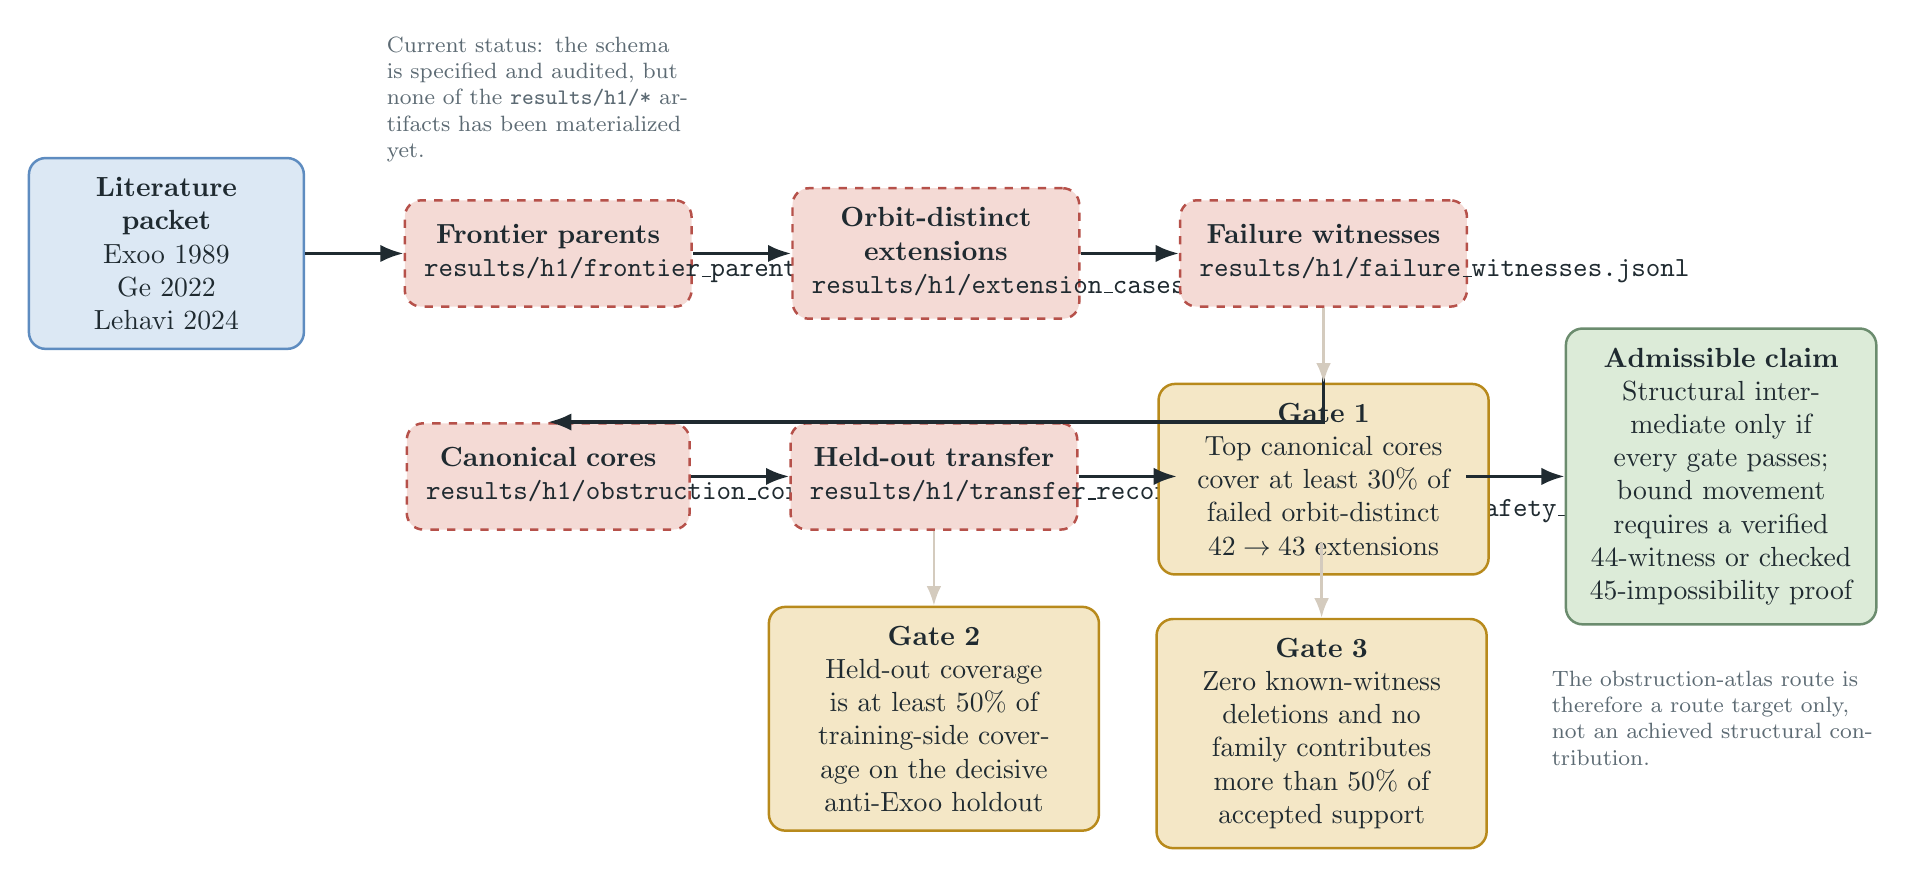
\begin{tikzpicture}[node distance=1.35cm and 1.25cm]
  \node[sourcebox, minimum width=3.35cm, text width=3.0cm] (lit)
    {\textbf{Literature packet}\\Exoo 1989\\Ge 2022\\Lehavi 2024};
  \node[missingbox, right=of lit, minimum width=3.4cm, text width=3.15cm] (parents)
    {\textbf{Frontier parents}\\\texttt{results/h1/frontier\_parents.jsonl}};
  \node[missingbox, right=of parents, minimum width=3.5cm, text width=3.15cm] (ext)
    {\textbf{Orbit-distinct extensions}\\\texttt{results/h1/extension\_cases.jsonl}};
  \node[missingbox, right=of ext, minimum width=3.5cm, text width=3.15cm] (wit)
    {\textbf{Failure witnesses}\\\texttt{results/h1/failure\_witnesses.jsonl}};

  \node[missingbox, below=1.45cm of parents, minimum width=3.4cm, text width=3.1cm] (cores)
    {\textbf{Canonical cores}\\\texttt{results/h1/obstruction\_cores.jsonl}};
  \node[missingbox, right=of cores, minimum width=3.5cm, text width=3.15cm] (transfer)
    {\textbf{Held-out transfer}\\\texttt{results/h1/transfer\_records.jsonl}};
  \node[missingbox, right=of transfer, minimum width=3.5cm, text width=3.15cm] (safety)
    {\textbf{Witness-safety audit}\\\texttt{results/h1/witness\_safety\_audit.md}};
  \node[successbox, right=of safety, minimum width=3.75cm, text width=3.45cm] (claim)
    {\textbf{Admissible claim}\\Structural intermediate only if every gate passes; bound movement requires a verified $44$-witness or checked $45$-impossibility proof};

  \node[gatebox, below=0.95cm of wit, minimum width=3.55cm] (gate1)
    {\textbf{Gate 1}\\Top canonical cores cover at least $30\%$ of failed orbit-distinct $42\!\to\!43$ extensions};
  \node[gatebox, below=0.95cm of transfer, minimum width=3.55cm] (gate2)
    {\textbf{Gate 2}\\Held-out coverage is at least $50\%$ of training-side coverage on the decisive anti-Exoo holdout};
  \node[gatebox, below=0.95cm of safety, minimum width=3.55cm] (gate3)
    {\textbf{Gate 3}\\Zero known-witness deletions and no family contributes more than $50\%$ of accepted support};

  \draw[stagearrow] (lit) -- (parents);
  \draw[stagearrow] (parents) -- (ext);
  \draw[stagearrow] (ext) -- (wit);
  \draw[stagearrow] (wit.south) |- (cores.north);
  \draw[stagearrow] (cores) -- (transfer);
  \draw[stagearrow] (transfer) -- (safety);
  \draw[stagearrow] (safety) -- (claim);

  \draw[faintarrow] (wit.south) -- (gate1.north);
  \draw[faintarrow] (transfer.south) -- (gate2.north);
  \draw[faintarrow] (safety.south) -- (gate3.north);

  \node[ann, above=0.35cm of parents, text width=4.1cm] {Current status: the schema is specified and audited, but none of the \texttt{results/h1/*} artifacts has been materialized yet.};
  \node[ann, below=0.45cm of claim, text width=4.3cm] {The obstruction-atlas route is therefore a route target only, not an achieved structural contribution.};
\end{tikzpicture}
\end{document}
